\documentclass[12pt,twoside]{article}
\usepackage{jmlda}
\usepackage[square,sort,comma,numbers]{natbib}
\usepackage{bm}
\usepackage{graphicx}
\newcommand{\cyrchar}[1]{\foreignlanguage{russian}{#1}}
\usepackage[labelfont=bf]{caption}
\usepackage{subfig} % for subfigures
\newcommand{\myfigref}[2]{~\ref{#1}.\subref{#2}}% <---- a new macro for referring to a subfigure
% \myfigref{label: fig}{label: subfig}

%\NOREVIEWERNOTES
\title
    [Предсказание показания фМРТ по видео, показанному человеку] % Краткое название; не нужно, если полное название влезает в~колонтитул
    {Предсказание показания фМРТ по видео, показанному человеку}
\author
    [Дорин~Д.\,Д.] % список авторов для колонтитула; не нужен, если основной список влезает в колонтитул
    {Дорин~Д.\,Д., Киселев~Н.\,С., Грабовой~А.\,В.} % основной список авторов, выводимый в оглавление
    [Дорин~Д.\,Д.$^{1,2}$, Грабовой~А.\,В.$^2$] % список авторов, выводимый в заголовок; не нужен, если он не отличается от основного

\email
    {dorin.dd@phystech.edu}
\organization
    {$^1$MIPT; $^2$Intelligent systems}
\abstract
    {Исследуется проблема восстановления зависимости между показаниями
    датчиков фМРТ и восприятием внешнего мира человеком. Проводится
    анализ зависимости между последовательностью снимков фМРТ и видеорядом, просматриваемым человеком. На основе исследования зависимости
    предлагается метод аппроксимации показаний фМРТ по просматриваемому видеоряду. Для анализа предложенного метода проводится вычислительный эксперимент на выборке, полученной при томографическом
    обследовании большого числа испытуемых.

\bigskip
\textbf{Ключевые слова}: \emph {фМРТ, видеоряд, Трансформер модель}.}
\titleEng
    {JMLDA paper example: file jmlda-example.tex}
\authorEng
    {Author~F.\,S.$^1$, CoAuthor~F.\,S.$^2$, Name~F.\,S.$^2$}
\organizationEng
    {$^1$Organization; $^2$Organization}
\abstractEng
    {This document is an example of paper prepared with \LaTexe\
    typesetting system and style file \texttt{jmlda.sty}.
    
\bigskip
\textbf{Keywords}: \emph{keyword, keyword, more keywords}.}

\begin{document}
\maketitle
%\linenumbers
\section{Введение}
Человеческий мозг~--- один из самых интересных объектов исследования \citep{Zhumakova}. 
Внутречерепные записи человека являются редким и ценным источником информации о мозге.
Поэтому изучение методов прогнозирования данных о функциональной активности коры головного мозга является актуальной темой в настоящее время.

Функциональная магнитно-резонансная томография, далее~--- фМРТ \citep{Ushakov},~--- один из методов исследования активности головного мозга.
фМРТ проводится с целью измерения гемодинамических реакций~--- изменений в потоке крови. 
Этот метод основывается на связи мозгового кровотока и активности нейронов. Когда область мозга активна, 
приток крови к этой области также увеличивается. 
фМРТ позволяет определить активацию определенной области головного мозга во время нормального функционирования под 
влиянием различных заданий, например, зрительных, когнитивных,  моторных,  речевых.
В работе \citep{Belyaevskaya2018} собраны современные возможности фМРТ в нейровизуализации. 
Под нейровизуализацией понимается общее название нескольких методов, позволяющих визуализировать структуру, функции и биохимические характеристики мозга.

В работе \citep{Berezutskaya2022} собран обширный набор данных, сотоящий из видеорядов, просмотренных 
человеком, и соответствующих снимков фМРТ. Одна из проблем при работе с данными нейровизуализации~--- шум, вызванный 
дивжением головы, биением сердца, тепловыми эффектами и др. 
В работе \citep{https://doi.org/10.48550/arxiv.1804.10167} рассмотрены подходы к подготовке,
предварительной обработке, шумоподавлению, направленные на устранение артефактов, вредных 
для распознавания образов, а также методы классификации данных нейровизуализации.

Наиболее известные методы обработки видео основаны на 3D свертках. 
Отличие 3D от 2D сверток заключается в одновременной работе с пространственной  
и временной частью информации. Существенный недостаток данных методов~--- 
сильное увеличение числа параметров модели и большие вычислительные затраты.
В работе используется более современная архитектура~--- модель типа Трансформер.
Впервые модель Трансформер была предложена в статье
\citep{https://doi.org/10.48550/arxiv.1706.03762}. Архитектура активно применяется в области машинного перевода.
А в 2022 году появилась работа \citep{transformer} на тему адаптации архитектуры Трансформер для работы с видеорядами. 
Данная архитектура учитывает пространственно-временные зависимости и повышает скорость обучения засчет механизма внимания.
Сама модель состоит из кодирующего компонента, декодирующего компонента и связи между ними. Каждый компонент состоит из стека 
энкодеров и декодеров соотвественно \citep{badrinarayanan2017segnet}. 
Входящая последовательность, поступающая в энкодер, сначала проходит через слой внимания, помогающий энкодеру 
посмотреть на другие слова во входящем объеме во время кодирования конкретного элемента. 
Выход слоя внимания отправляется в нейронную сеть прямого распространения. 
Аналогично устроен декодер, за исключением наличия еще одного слоя внимания, помогающего фокусироваться на релевантных элементах.

В данной работе предлагается метод аппроксимации показаний датчиков фМРТ по видеоряду. 
При получении метода используются два основных предположения. Первая гипотеза заключается в существовании зависимости между результатами фМРТ и просматриваемым фильмом.
Второе предположение заключается в том, что реакция мозга, фиксируемая фМРТ, на информацию, поступающую от органов зрения, происходит не мгновенно, а с некоторой задержкой \citep{Demidov}. 
Полученная в ходе экспериментов корреляционная картина между данными в выборке подтверждает 
зависимость между показаниями фМРТ и восприятием внешнего мира человеком. 

Проверка метода проводится на выборке, представленной в работе \citep{Berezutskaya2022}. 
Набор данных включает в себя в себя записи фМРТ 30 участников в возрасте от 7 до 47 лет во время 
выполнения одинаковой задачи и записи внутричерепной электроэнцефалографии 51 участникa в возрасте от 5 до 55 лет. 


\section{Постановка задачи}
Пусть $\bm{\mathcal{P}}$~--- видеоряд, $\nu$~--- частота кадров, $t$~--- продолжительность видеоряда:
\begin{equation}
    \bm{\mathcal{P}} = (\bm{p}^{1}, \dots, \bm{p}^{\nu \cdot t}),
\end{equation}
где $\bm{p} \in \mathbb{R}^{W_{\bm{p}} \times H_{\bm{p}} \times C_{\bm{p}}}$~--- изображение, $W_{\bm{p}}$~---
ширина изображения, $H_{\bm{p}}$~--- высота изображения и $C_{\bm{p}}$~--- число каналов.

Введем также $\mathcal{S}$~--- последовательность фМРТ снимков,  $\mu$~--- частота снимков:
\begin{equation}
    \mathcal{S} = (\bm{s}^{1}, \dots, \bm{s}^{\mu \cdot t}),
\end{equation}
где $\bm{s} \in \mathbb{R}^{X_{\bm{s}} \times Y_{\bm{s}} \times Z_{\bm{s}}}$~--- фМРТ снимок, $X_{\bm{s}},~Y_{\bm{s}},~Z_{\bm{s}}$~--- размерности тензора снимка фМРТ.


Также считаем, что известно несколько дополнительных измерений фМРТ $\mathcal{S}_0$ того же испытуемого.
Необходимо построить отображение $\bm{f}$:
\begin{equation}
    \bm{f}(\bm{p}^{1}, \dots, \bm{p}^{k_i - \nu \cdot \Delta t}, \mathcal{S}_0) = \bm{s}^i,
\end{equation}
которое учитывает задержку $\Delta t$, между фМРТ картиной и моментом получения информации зрительными органами.
Здесь
\begin{equation}
    \label{k_i}
    k_i = \dfrac{\nu \cdot i}{\mu}
\end{equation}
номер изображения в момент времени $i$-го снимка фМРТ.

\section{Описание модели}
Пусть имеется набор данных некотрого испытуемого, состоящий из $L$ снимков фМРТ и соотвествующего этим снимкам видеоряда.
Для каждого фиксированного гиперпараметра $\Delta t$ выборка состоит из $L_{\Delta t} = L - \mu \cdot \Delta t$  снимков фМРТ и набора соотвествующих изображений из видеоряда. 
Номера изображений определяются по номеру снимка фМРТ соотвественно формуле:
\begin{equation}
    k_i - \nu \cdot \Delta t,
\end{equation}
где $k_i$ определен по формуле \eqref{k_i}, $i$~--- номер изображения соотвественно.

Будем работать в предположении, что каждый снимок фМРТ зависит только от одного изображения и предыдущего снимка фМРТ. 
То есть будем предсказывать разницу между фМРТ показаниями, что позволит учесть временную зависимость между снимками.
Тогда отображение имеет вид:
\begin{equation}
	\label{main_model}
	\bm{f}(\bm{p}^{k_i - \nu \cdot \Delta t}) = \bm{\delta}^i, \ i = 2, \ldots, L_{\Delta t},
\end{equation}
где $\bm{\delta}^i = \bm{s}^i - \bm{s}^{i-1},~\bm{s}^k \in \mathbb{R}^{X_{\bm{s}} \times Y_{\bm{s}} \times Z_{\bm{s}}}$~--- тензор снимка фМРТ под номером $k$.
Обозначим $\delta_{ijk}$~--- компонента разницы между тензорами снимков $\bm{\delta}$.
Каждое изображения $\bm{p}$ из обучающей выборки предобработано с помощью ResNet152 без последнего линейного слоя и представляет собой вектор $\bm{x}$ признаков размерности $d$:
\[ \bm{x}^i = [x^i_1, \ldots, x^i_{d}]^{T} \in \mathbb{R}^{d}, \ i = 1, \ldots, K, \]
где $K$ общее число изображений в видеоряде.

Для восстановления разности значений в каждом вокселе с течением времени по всему признаковому вектору изображения используется линейная модель. Вектор параметров имеет вид:
\[ \bm{w}_{ijk} = [w_{ijk}^1, \ldots, w_{ijk}^{d}]^{T} \in \mathbb{R}^{d}: \]
\begin{equation}
	\label{f_ijk}
	f_{ijk}(\bm{x}, \bm{w}_{ijk}) = \langle \bm{x}, \bm{w}_{ijk} \rangle.
\end{equation}

Для каждого вокселя в снимке задана обучающая выборка:
\begin{equation}
    \mathcal{D}_{ijk} = \left(\bm{x}^l,~\delta^{l}_{ijk} \right)^{ L_{\Delta t}}_{l = 2}
\end{equation}
Выборка делится на тренировочную и тестовую в соотношении $7 : 3$. 
Обозначим число объектов тренировочной выборки $N$.

Для модели $f_{ijk}$, с соответствующей ей тренировочной выборкой,
определим квадратичную функцию потерь с $L_2$ регуляризатором:
\begin{equation}
	\label{Loss}
	\mathcal{L}_{ijk}(\bm{w}_{ijk}, \Delta t, \alpha) = \frac{1}{2} \sum\limits_{l = 2}^{N+1} \big(f_{ijk}(\bm{x}^l, \bm{w}_{ijk}) - \delta^{l}_{ijk}\big)^2 + \frac{\alpha}{2} \|\bm{w}_{ijk}\|^2_2.
\end{equation}

Требуется минимизировать функцию потерь $\mathcal{L}_{ijk}(\bm{w}_{ijk}, \Delta t, \alpha)$ при фиксированных гиперпараметрах $\Delta t$ и $\alpha$:
\begin{equation}
	\label{main_Problem}
	\hat{\bm{w}}_{ijk} = \argmin_{\bm{w}_{ijk}} \mathcal{L}_{ijk}(\bm{w}_{ijk}, \Delta t, \alpha).
\end{equation}

Определим матрицу объектов тренировочной выборки
\begin{equation}
\label{X}
    \bm{X} = [{\bm{x}^2}^T, \dots, {\bm{x}^{N+1}}^T]^T = [x^i_j] \in \mathbb{R}^{N \times d}
\end{equation}
и вектор, компонентами которого являются разности значений одного и того же вокселя в снимках тренировочной выборки,
\begin{equation}
\label{Delta}
    \bm{\Delta}_{ijk} = [\delta^{2}_{ijk}, \dots, \delta^{N+1}_{ijk}]^T \in \mathbb{R}^{N}.
\end{equation}
Тогда решение можно записать в виде:
\begin{equation}
\label{weights}
    \hat{\bm{w}}_{ijk} = (\bm{X}^T \bm{X} + \alpha \mathbf{I})^{-1} \bm{X}^T \mathbf{\Delta}_{ijk}.
\end{equation}

Веса, полученные согласно формуле \eqref{weights} для каждого вокселя снимка, запишем в виде строк матрицы весов
\begin{equation}
\label{matrix_weights}
    \hat{\bm{W}} = [\hat{\bm{w}}_1^T, \dots, \hat{\bm{w}}_{X_{\bm{S}} \cdot Y_{\bm{S}} \cdot Z_{\bm{S}}}^T]^T = [w^i_j] \in \mathbb{R}^{X_{\bm{S}} \cdot Y_{\bm{S}} \cdot Z_{\bm{S}} \times d}.
\end{equation}
Тогда предсказание разности значений вокселей соседних снимков в виде вектора $\hat{\bm{{V_{\delta}}}}^l$ можно вычилсить по следующей формуле:
\begin{equation}
\label{Vector_delta}
    \hat{\bm{{V_{\delta}}}}^l = \hat{\bm{W}} \cdot \bm{x}_l \in \mathbb{R}^{X_{\bm{S}} \cdot Y_{\bm{S}} \cdot Z_{\bm{S}}}.
\end{equation}
Произведем reshape $\hat{\bm{{V_{\delta}}}}^l$ к тензору $\hat{\bm{\delta}}^l$. Тогда предсказанный тензор снимка фМРТ $\hat{\bm{s}}^l$ под номером $l$ может быть получен согласно формуле:
\begin{equation}
    \label{Vector_delta}
    \hat{\bm{s}}^l = \hat{\bm{\delta}}^l + \bm{s}^{l-1},
\end{equation}
где $\bm{s}^{l-1}$ оригинальный тензор снимка фМРТ под номером $l-1$.


Одним из параметров модели является коэффициент сжатия воксельных снимков фМРТ. 
Рассматриваются коэффициенты сжатия 1, 2, 4 и 8.
Для сжатия используется MaxPool3d с целью уменьшения числа подбираемых весов и ускорения процесса обучения соотвественно.
Метрикой оценки качества алгоритма ялвяется среднеквадратичная ошибка.
Усреднение берется по всем вокселям снимков фМРТ и по всем снимкам в тестовой выборке.


\section{Вычислительный эксперимент}
\subsection{Цель эксперимента}
Проверить корректность предложенного метода, оценить качество работы метода на тестовых данных и проверить основные гипотезы.
\subsection{Набор данных для эксперимента}
Набор данных для эксперимента, представленный в работе \citep{Berezutskaya2022}, состоит из снимков фМРТ и видеорядов тридцати испытуемых. 
Для обучения модели выбирается набор данных одного из испытуемых. 


Частоты изображений и снимков фМРТ соотвественно имеют значения $\nu = 25~с^{-1},~\mu = 1.64~с^{-1}$.
Число снимков фМРТ в выборке $L = 641$.  
Для каждого фиксированного гиперпараметра $\Delta t$ выборка состоит из $L_{\Delta t} = 641-\mu \cdot \Delta t$  снимков фМРТ и набора соотвествующих изображений из видеоряда. 
Каждый снимков фМРТ представляет тензор $\bm{s} \in \mathbb{R}^{{40} \times {64} \times {64}}$.
Изображения из видеоряда представляют собой тензоры $\bm{p} \in \mathbb{R}^{{640} \times {480} \times {3}}$.
После предобработки изображений из видеоряда с помощью ResNet152 без последнего линейного слоя они представляет собой вектора признаков размерности $d = 2048$. 
Общее число изображений в видеоряде $K = 9750$.

\subsection{Демонстрация работы алгоритма}
В качестве демонстрации работы алгоритма на Рис.\ref{fig:5} приведены срезы оригинального и предсказанного воксельного снимка фМРТ из тестовой выборки.
\begin{figure}[h!]
    \centering
    \subfloat[Истинный]{\label{fig:5a}{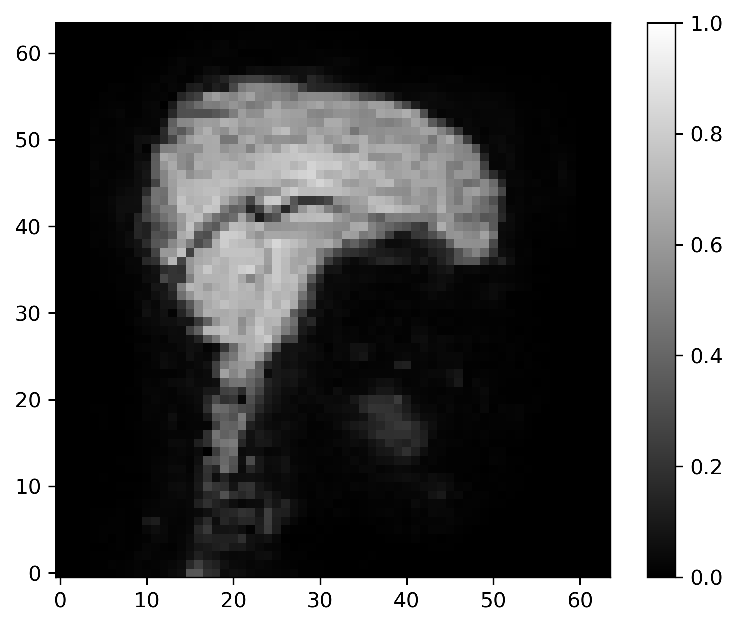
\includegraphics[width=0.33\textwidth]{sub-04-5-1-1000-100-20-_-_-test.pdf}}}
    \hfill
    \subfloat[Восстановленный]{\label{fig:5b}{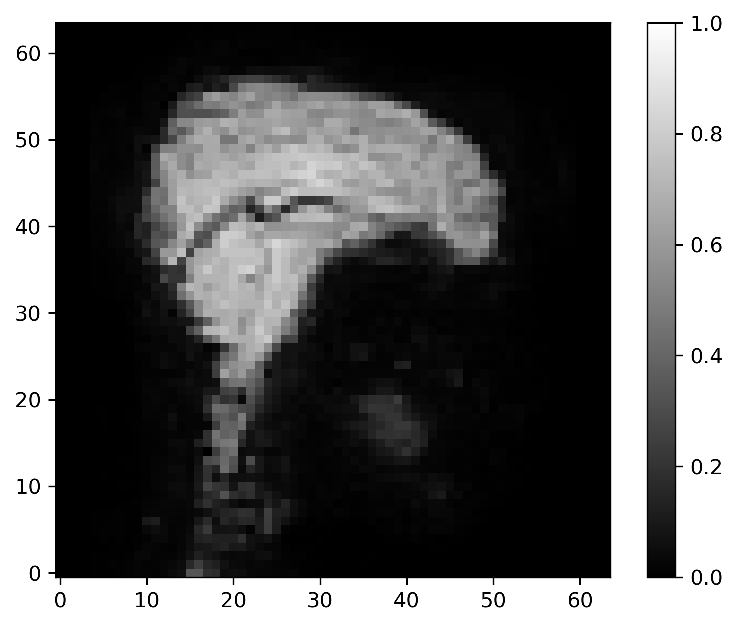
\includegraphics[width=0.33\textwidth]{sub-04-5-1-1000-100-20-_-_-predicted.pdf}}}
    \hfill
    \subfloat[Разность]{\label{fig:5c}{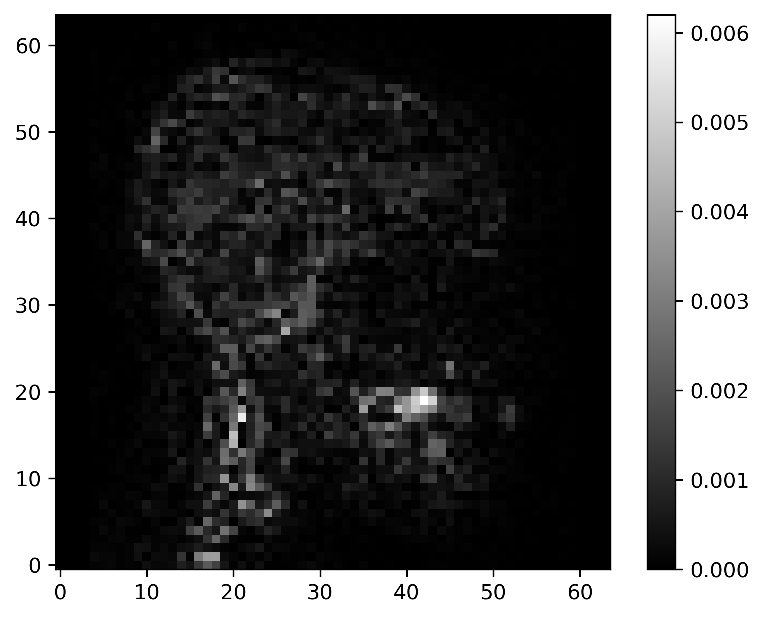
\includegraphics[width=0.33\textwidth]{sub-04-5-1-1000-100-20-_-_-difference.pdf}}}
    \caption{Срез снимка фМРТ из тестовой выборки}
    \label{fig:5}
\end{figure}
Ошибка порядка $10^{-3}$ в отдельных вокселях говорит о хорошем качестве работы алгоритма.

\section{Анализ ошибки}
\subsection{Варьирование гиперпараметров}
На Рис.\ref{MSE_dt_main} приведены результаты работы модели при варьировании гиперпараметра $\Delta t$, усредненные по всем испытуемым из выборки. Здесь фиксирован коэффициент сжатия $\mathrm{coef} = 8$ и гиперпараметр регуляризации $\alpha = 100$. Фоном демонстрируется среднеквадратичное отклонение от среднего.
\begin{figure}[h!]
    \centering
    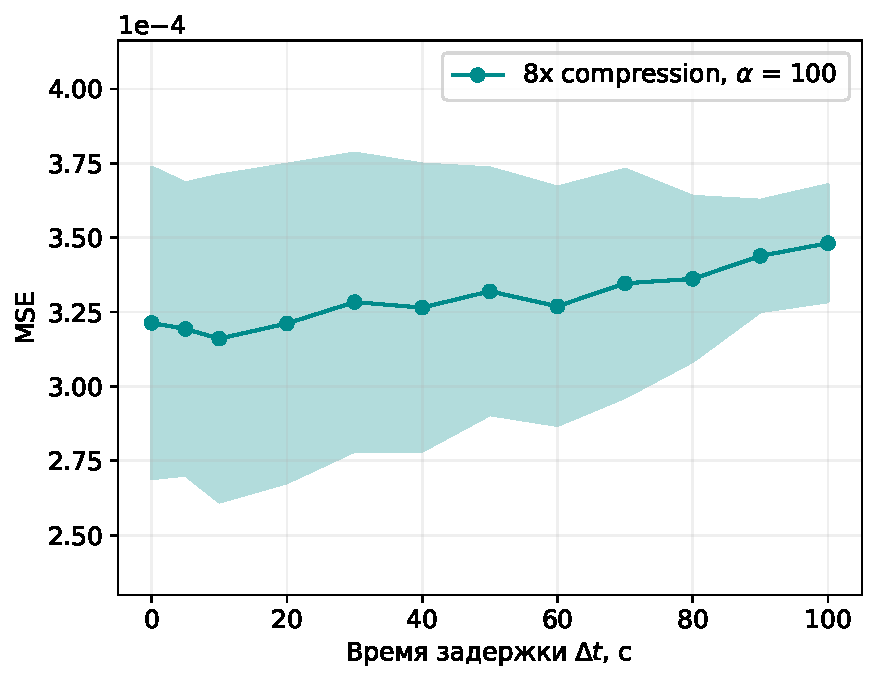
\includegraphics[width=0.65\textwidth]{subs_delta_MSE_dt.pdf}
    \caption{Зависимость среднеквадратичной ошибки на тесте от задержки ${\Delta t}$}
    \label{MSE_dt_main}
\end{figure}
График демонстрирует наличие зависимости результата предсказания от гиперпараметра $\Delta t$. 
Причем при нефизичной задержке больше десяти секунд ошибка начинает расти. 
Минимум достигается в пределах 4~---10 секунд, что хорошо согласуется с нейробиологическими сведениями.

Проанализированна зависимость MSE от коэффициента регуляризации $\alpha$.
Рассматриваются коэффициенты сжатия 1, 2, 4 и 8. 
Соответствующие графики приведены на Рис.~\ref{subs_MSE_alpha}.
\begin{figure}[h!]
    \centering
    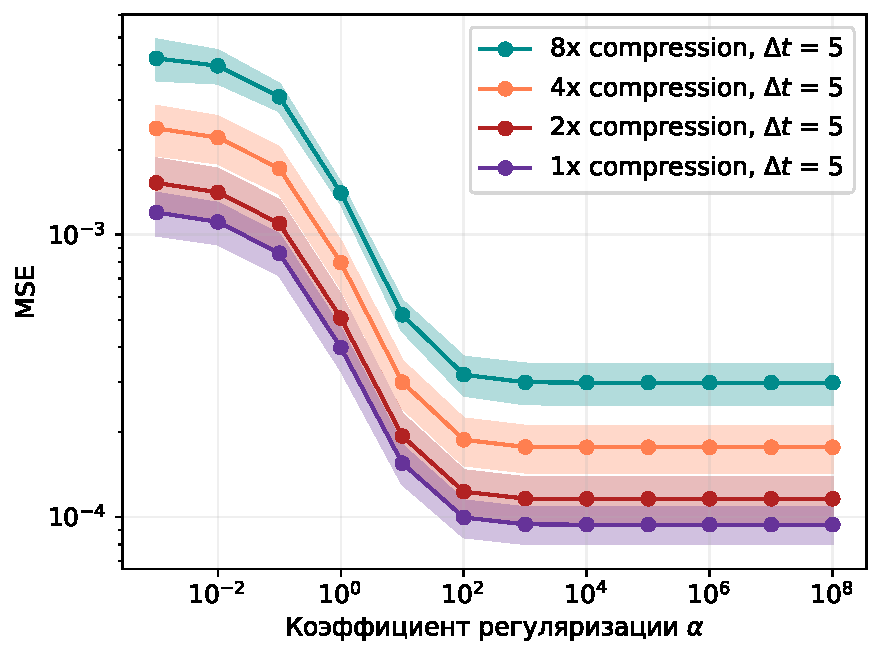
\includegraphics[width=0.65\textwidth]{subs_MSE_alpha.pdf}
    \caption{Зависимость среднеквадратичной ошибки на тесте от коэффициента регуляризации $\alpha$}
    \label{subs_MSE_alpha}
\end{figure}
Из графиков видно, что отстуствие регуляризации ведет к переобучению модели.
Оптимальное значение коэффициента $\alpha \approx 100$.


\subsection{Корректность алгоритма}
На Рис.\ref{fig:6} приведено распределения значений компонент вектора весов модели. 
Для построения производилось усреднение по строкам матрицы весов $\hat{W}$, то есть усреднение по всем вокселям.
График на Рис.\ref{fig:6} хорошо аппроксимируется плотнотью нормального распределения, что говорит о статистической значимости весов.
\begin{figure}[h!]
    \centering
    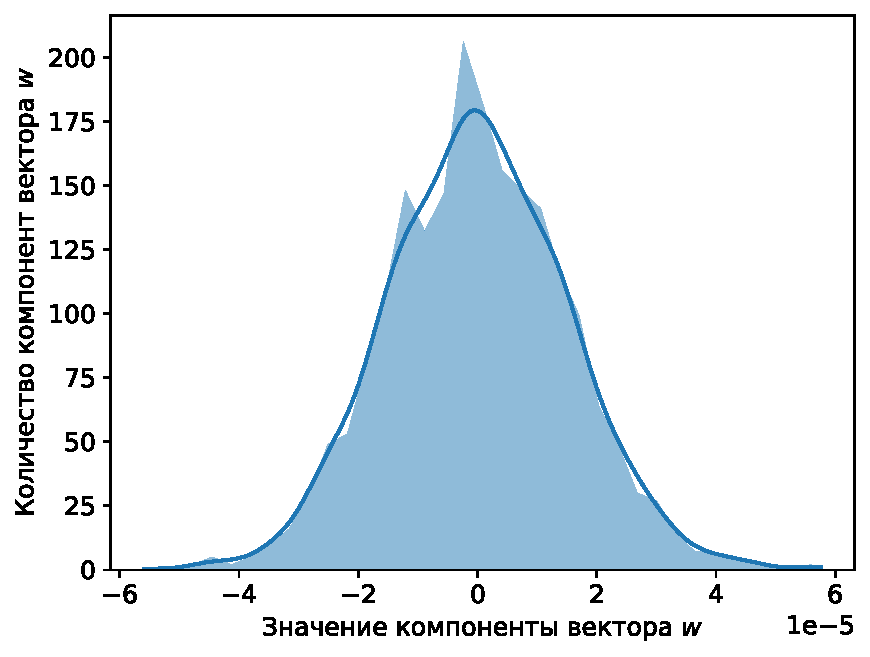
\includegraphics[width=0.65\textwidth]{mean_weight_distribution.pdf}
    \caption{Распределение значений компонент вектора весов}
    \label{fig:6}
\end{figure}

Экспериментально проверено, что модель улавливает общие для всех испытуемых зависимости между данными.
Другими словами, восстановление снимка фМРТ одного человека можно производить, используя
матрицу весов другого испытуемого. 
Для оценки качества работы алгоритма в данном эксперименте использовалась метрика MSE на тестовой выборке.
Результаты представлены в Таблице~\ref{table_2}.

	\begin{table}[h!]
		\centering
		\begin{tabular}{|c|c|c|}
			\hline
			Матрица весов	&	Истинная	&	Подмешанная \\ \hline \hline
			MSE		& 	$1.02 \cdot 10^{-4}$	 &		$1.05 \cdot 10^{-4}$ \\ \hline
		\end{tabular}
		\caption{Проверка гипотезы инвариантности весов модели относительно человека}
		\label{table_2}
	\end{table}

Ниже приведены результаты работы модели на случайном шуме. 
Первоначально модель обучена на оригинальных изображениях из видеоряда.
Получена соответствующая матрица весов $\hat{W}$. 
К первому снимку последовательно прибавляются все восстановленные изменения значений вокселей. 
В результате имеем последний снимок последовательности. На Рис.~\ref{fig:7} представлены срезы последнего истинного и восстановленного снимков из тестовой выборки.
Для демонстрации работы на случайном шуме сгенерирована случайная выборка из векторов признакового описания изображения размера тестовой выборки.
По шумовым данным и матрице весов $\hat{W}$ получена последовательность изменений между соседними снимками фМРТ. 
Аналогично последнему снимку, полученному по оригинальным изображениям, предсказан последний снимок по шуму. 
На Рис.~\ref{fig:8} представлены срезы последнего истинного и восстановленного по шуму снимков из тестовой выборки.
\begin{figure}[h!]
    \centering
    \subfloat[Истинный]{\label{fig:7a}{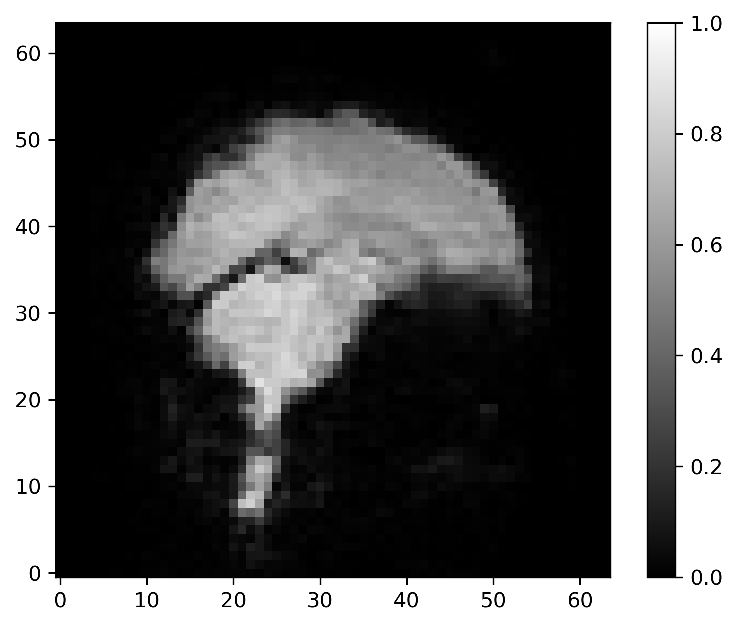
\includegraphics[width=0.33\textwidth]{sub-35-5-1-1000--1-20-_-_-recovered-test.pdf}}}
    \hfill
    \subfloat[Восстановленный]{\label{fig:7b}{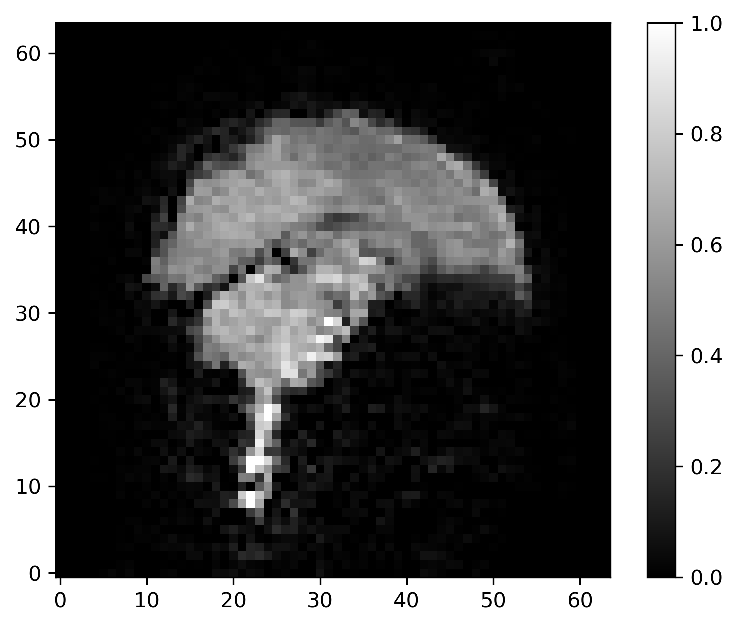
\includegraphics[width=0.33\textwidth]{sub-35-5-1-1000--1-20-_-_-recovered-predicted.pdf}}}
    \hfill
    \subfloat[Разность]{\label{fig:7c}{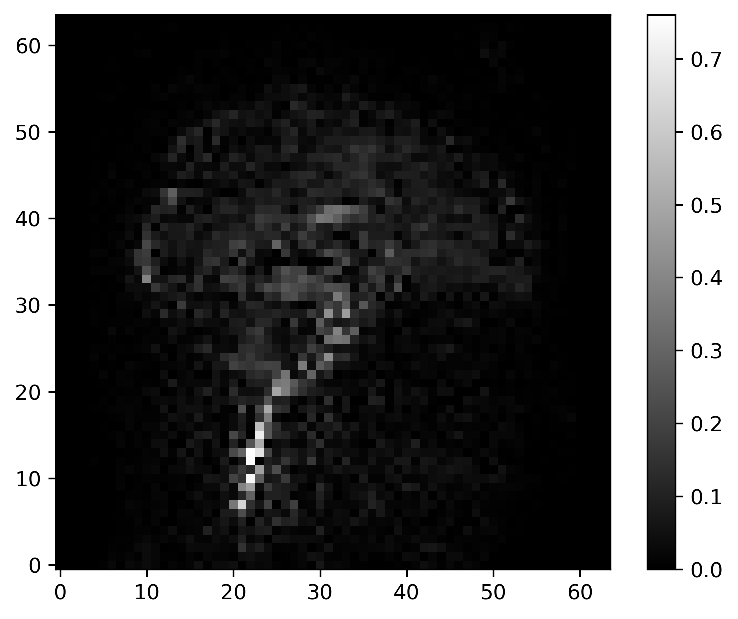
\includegraphics[width=0.33\textwidth]{sub-35-5-1-1000--1-20-_-_-recovered-difference.pdf}}}
    \caption{Срез снимка фМРТ из тестовой выборки}
    \label{fig:7}
\end{figure}

\begin{figure}[h!]
    \centering
    \subfloat[Истинный]{\label{fig:8a}{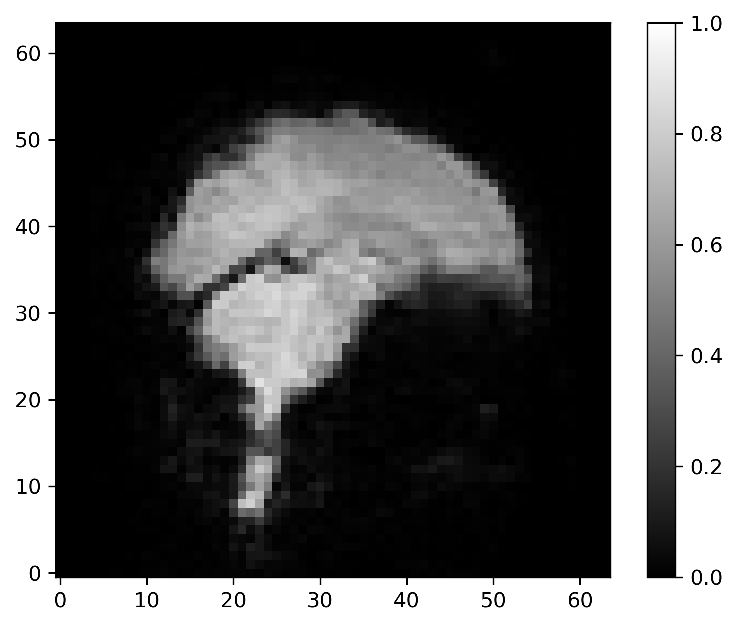
\includegraphics[width=0.33\textwidth]{sub-35-5-1-1000--1-20-_-_-recovered-test_noised.pdf}}}
    \hfill
    \subfloat[Восстановленный по шуму]{\label{fig:8b}{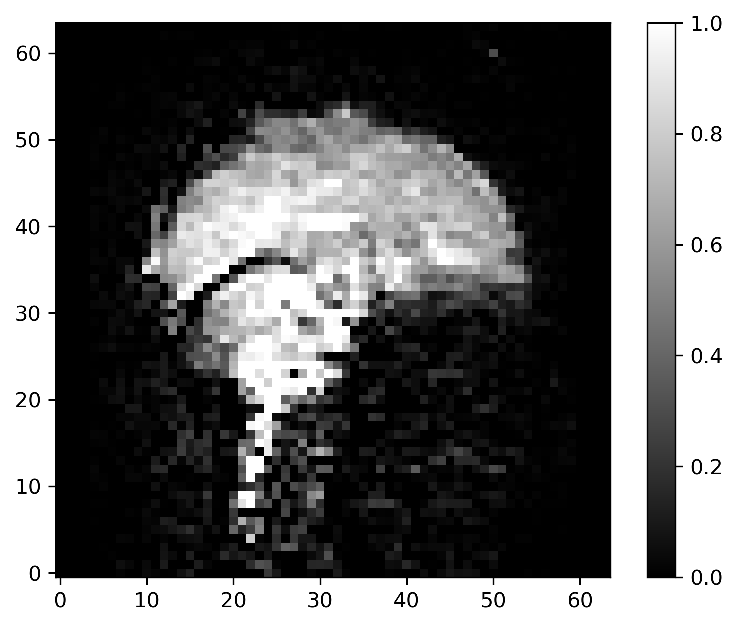
\includegraphics[width=0.33\textwidth]{sub-35-5-1-1000--1-20-_-_-recovered-predicted_noised.pdf}}}
    \hfill
    \subfloat[Разность]{\label{fig:8c}{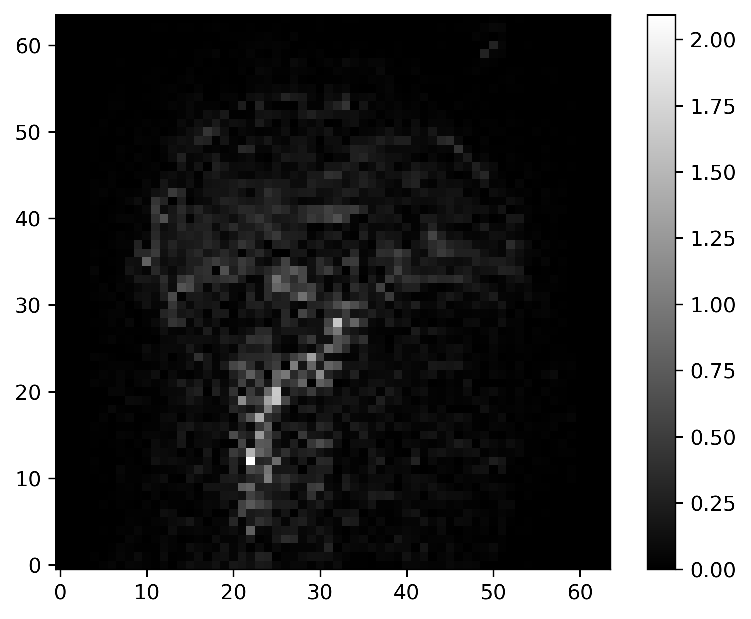
\includegraphics[width=0.33\textwidth]{sub-35-5-1-1000--1-20-_-_-recovered-difference_noised.pdf}}}
    \caption{Срез снимка фМРТ из тестовой выборки на случайном шуме}
    \label{fig:8}
\end{figure}
На приведенных изображениях можно видеть, что разность в случе шума существенно больше.
В таблице \ref{table_3} приведены среднеквадратичные ошибки.
Ошибка на шуме на порядок больше, что подтверждает наличие корреляции между показаниями датчиков и изображениями из видеоряда.
\begin{table}[h!]
    \centering
    \begin{tabular}{|c|c|c|}
        \hline
        Выборка	&	Истинная	&	Случайный шум \\ \hline \hline
        MSE		& 	$2 \cdot 10^{-3}$	 &		$10^{-1}$ \\ \hline
    \end{tabular}
    \caption{Качество работы метода на случайном шуме}
    \label{table_3}
\end{table}

\section{Заключение}
В работе построен метод аппроксимации показаний датичков фМРТ по видеоряду, просматриваемому человеком. 
Результаты эксперимента со случайным шумом подтверждают наличие корреляции между данными.
В работе экспериментально подтверждено, что веса модели инвариантны относительно человека. 
График распределения значений компонент весов модели хорошо аппроксимируется нормальным распределением, что говорит о статистической значимости весов.
График, полученный при варьировании $\Delta t$, подтверждает предположение о наличии задержки между моментом получения информации зрительными органами и реакцией мозга на эту информацию.

 
\newpage
\bibliographystyle{plain}

\bibliography{dorin.bib}

%\begin{thebibliography}{1}

%\bibitem{author09anyscience}
%    \BibAuthor{Author\;N.}
%    \BibTitle{Paper title}~//
%    \BibJournal{10-th Int'l. Conf. on Anyscience}, 2009.  Vol.\,11, No.\,1.  Pp.\,111--122.
%\bibitem{myHandbook}
%    \BibAuthor{Автор\;И.\,О.}
%    Название книги.
%    Город: Издательство, 2009. 314~с.
%\bibitem{author09first-word-of-the-title}
%    \BibAuthor{Автор\;И.\,О.}
%    \BibTitle{Название статьи}~//
%    \BibJournal{Название конференции или сборника},
%    Город:~Изд-во, 2009.  С.\,5--6.
%\bibitem{author-and-co2007}
%    \BibAuthor{Автор\;И.\,О., Соавтор\;И.\,О.}
%    \BibTitle{Название статьи}~//
%    \BibJournal{Название журнала}. 2007. Т.\,38, \No\,5. С.\,54--62.
%\bibitem{bibUsefulUrl}
%    \BibUrl{www.site.ru}~---
%    Название сайта.  2007.
%\bibitem{voron06latex}
%    \BibAuthor{Воронцов~К.\,В.}
%    \LaTexe\ в~примерах.
%    2006.
%    \BibUrl{http://www.ccas.ru/voron/latex.html}.
%\bibitem{Lvovsky03}
%    \BibAuthor{Львовский~С.\,М.} Набор и вёрстка в пакете~\LaTex.
%    3-е издание.
%    Москва:~МЦHМО, 2003.  448~с.
%\end{thebibliography}

% Решение Программного Комитета:
%\ACCEPTNOTE
%\AMENDNOTE
%\REJECTNOTE
\end{document}
